\chapter{Direct Detection of Dark Matter}
\label{chap:detection_theory}
\par
We have seen in the previous chapter that both there is a wealth of evidence for some particle or particle combination that is missing from our understanding of particle physics.
Equally there are just as many proposed solutions.
In this Chapter, we focus on WIMPs that were introduced in \autoref{sec:wimp_as_a_candidate}, and how they might be detected in direct dark matter experiments.


\section{WIMP-nucleon interactions} \label{sec:wimp_nucleus_interactions}
\iffalse
\par
As WIMPs travel at relative non-relativistic speeds, the recoil energy of the nucleon resulting from an elastic scatter is by only the centre of mass scattering angle, $\theta$ \cite{direct_detection_of_wimps_ref}:
\begin{equation}
    E_{R} = \frac{{\mu}_{N}^{2}\nu_{\chi}^2}{m_{N}}(1-\cos(\theta))
\end{equation}
\fi
Direct dark matter detectors are built on the principle of having a large mass of material on which a WIMP can scatter \cite{direct_detection_of_wimps_ref}.
Within a detector, the rate of these WIMP scatter interactions, $R$, is given by:
\begin{equation}
    R = \sigma N_{T} n_{\chi} \langle v \rangle
    \label{eq:wimp_nucleon_rate}
\end{equation}
where N$_{T}$ is the number of nuclei in the detector, $n_\chi$ is the number density of dark matter particles travelling with an average speed $\langle v \rangle$ relative to the target, and $\sigma$ is the interaction cross-section, representing the interaction strength between the dark matter and the nucleus.
\par
Given that each direct detector is sensitive to different recoil energies depending upon the design, it is beneficial to describe the event rate in an energy region as the differential scattering rate with respect to recoil energy \cite{supersymetry_wimpy_boi_ref}:
\begin{equation}
\begin{split}
    \frac{dR}{dE_R} &= \frac{\rho_{\chi}}{m_\chi m_A} \int^{\infty}_{v_{min}} v f(\vec{v}) \frac{d\sigma}{dE_R} d\vec{v} \\
                    &= \frac{2\rho_{\chi}}{m_\chi} \int^{\infty}_{v_{min}} v f(\vec{v}) \frac{d\sigma}{d |q|^2} d\vec{v}
\end{split}
\label{eq:wimp_differential_rate}
\end{equation}
where $f(\vec{v})$ is the dark matter velocity distribution in the galactic halo, $\rho_{\chi}$ is the dark matter density, $m_\chi$ is the dark matter mass, $m_A$ is the target nucleus mass, and $q$ is the momentum transfer associated with the recoil given by $q = \sqrt{2m_A E_R}$ and $v_{min}$ is the minimum velocity of dark matter to induce a recoil of energy $E_R$.
It is therefore a detector specific limit given by $v_{min} = \sqrt{(m_\chi E_R)/(2\mu^2)}$ where $\mu = (m_\chi m_A)/(m_\chi + m_A)$, the WIMP-nucleus reduced mass.
\par
We are able to control the detector size and target properties (within reason).
This leaves us with two parameters outside of our direct control but which we need to constrain in order to determine an expected rate in any given detector: the dark matter velocity distribution and the differential cross-section.

\subsection{Local Astrophysical Dark Matter Properties}
\par
The standard dark matter model has two parameters that need to be determined experimentally: the velocity distribution and the density. 
Both have sufficient uncertainties to significantly impact the sensitivity of any direct detection experiment \cite{local_dm_uncertainties_ref}.
\par
The local dark matter density has long been studied, with the earliest references from 1922 \cite{first_dm_density_1_ref, first_dm_density_2_ref}.
Since then, many measurements have been done which constrain $\rho_{\chi}$.
These fall into two categories: galactic measurements and local measurements \cite{dm_density_ref}.
Galactic measurements derive $\rho_{\chi}$ from rotation curves, which does not require the assumption of a galactic halo.
Local measurements typically observe tracer star motion near the Sun \cite{gaia_tracer_dm_density_ref}.
Naturally there is variation in these two approaches where the galactic measures place $\rho_{\chi}$ in the range 0.2-0.6 GeV/cm$^3$ whilst the latest result from Gaia \cite{gaia_data_2_ref} have $\rho_{\chi}$ between 0.1-1.5 GeV/cm$^3$ \cite{gaia_dm_density_2_ref}.
Prior to the second data release of Gaia, the best-fit of all the studies lay in the range 0.22-0.33 GeV/cm$^3$, as such $\rho_{\chi}$ has typically been taken to be 0.3 GeV/cm$^3$.
This may change in the coming years as the current best-fit from Gaia studies suggest $\rho_{\chi}=0.5$ GeV/cm$^{3}$ \cite{gaia_dm_density_1_ref}.
\par
With regard to the velocity distribution, there are a number of models that are often used. 
Including simple isotropic models \cite{isotropic_dark_matter_models_ref}, isothermal sphere dark matter \cite{dm_velocity_isothermal_ref} and the Standard Halo Model (SHM) \cite{dm_velocity_shm_ref}. 
We shall only consider the SHM here as it is the most common choice \cite{dark_matter_distribution_models_ref}.
\par
In the SHM, a Maxwell-Boltzmann velocity distribution is assumed, which is truncated at the escape velocity ($v_{\text{esc}}$) of the Milky Way \cite{direct_dark_matter_of_wimps_concepts_ref}.
This constrains the dark matter to be within the galaxy.
The SHM also assumes dark matter is isotropic and spherically symmetrically distributed in the galaxy\footnote{The distribution is not perfectly symmetrical, and there are newer models referred to as SHM$^{++}$ which try and account for this, but they are not considered here \cite{extended_shm_ref}}.
The velocity distribution of dark matter within the Milky Way halo in the Earth frame is approximated as \cite{direct_dark_matter_of_wimps_concepts_ref, shm_derivation_ref}:
\begin{equation}
    f(\vec{v}) = \frac{1}{k} e^{\frac{- (\vec{v} - \vec{v}_E)^2 }{ v^2_0} }
    \label{eq:shm_short_equation}
\end{equation}
where $\vec{v}$ is the velocity of the dark matter with respect to the Earth, $\vec{v}_E$ is the velocity of the Earth around the centre of the galaxy and $\vec{v}_0$ is the peculiar velocity of the Sun relative to its circular velocity. 
\autoref{eq:shm_short_equation} is only valid for when $|\vec{v} + \vec{v}_E| < v_{\text{esc}}$.


%\begin{equation}
% f(\vec{v}) = \frac{1}{(2\pi\sigma^2_{v})^{\frac{3}{2}}N_{esc}} e^{\frac{- |\vec{v}|^2}{2\sigma^2_v}} \Theta(v_{esc} - |\vec{v}|)
%\label{eq:shm_velocity_1}
%\end{equation}
%where $\Theta$ is a Heaviside step function, $\sigma_v$ is the velocity dispersion, and .
%
%\par
%The dark matter velocity distribution which was used in \autoref{eq:wimp_differential_rate_scattering_amplitude} was normalised such that $\int f(\vec{v}) dv = 1$.
%As such we need to renormalise \autoref{eq:shm_velocity_1} to allow for the integral of $\sigma_{v}$ to be unitary as well.
%We do this by:
%\begin{equation}
%    N_{esc} = erf(z) - 2z e^\frac{-z^2}{\pi^{\frac{1}{2}}}
%\end{equation}
%where erf is the error function (given by $\text{erf}(z) = 2/\sqrt{\pi}\int^{z}_{0} e^{-t^2} dt$) and $z=v_{esc}/v_0$.
%We also need to define two other variables: $x=v_{min}/v_{0}$ and $y=|V_E|/v_0$ where $|V_E|$ is the velocity of the Earth with respect to the dark matter halo.
%Using these we can define our integral as \cite{shm_derivation_ref}:
%\begin{equation}
%\begin{split}
% \int \frac{f(\vec{v})}{v} = 
%\begin{dcases}
%\frac{1}{v_0 y}  & \text{if}\; z<y,x<|y-z| \\
%\frac{1}{2N_{esc} v_{0}y} \bigg[\text{erf}(x+y) - \text{erf}(x-y) - \frac{4}{\sqrt{\pi}}ye^{-z^2} \bigg] & \text{if}\; z>y, x<|y-z| \\
%\frac{1}{2N_{esc} v_{0}y} \bigg[\text{erf}(z) - \text{erf}(x-y) - \frac{2}{\sqrt{\pi}}(y + z - x)e^{-z^2} \bigg] & \text{if}\; |y-z|<x<|y+z|
%\end{dcases}
%\end{split}
%\label{eq:shm_velocity_2}
%\end{equation}
\par
Depending upon the values used for both the dark matter density and the velocities, the scattering rate will vary, and therefore the sensitivity of any given experiment will vary.
Historically the parameters used for determining the event rate have varied between experiments, making comparisons between results difficult.
However, recent collaboration between dark matter experiments have now agreed upon a common set of parameters \cite{standard_halo_model_conventions_ref} summarised in \autoref{tab:standard_parameters_for_dm}.
For a review of how these affect sensitivity to a dark matter discovery, the reader is directed to \cite{dm_velocity_effects_on_limits_ref}.

\begin{table}[]
    \centering
    \begin{tabular}{c|c|c}
        Parameter                               & Description                       & Value         \\ \hline
        $\rho_{\chi}$                           & Local dark matter density         & 0.3 GeV/cm$^2$ \cite{shm_derivation_ref}           \\
        $v_{esc}$                             & Galactic escape velocity          & 544 km/s  \cite{dm_v_esc_ref}           \\
        $v_0$                             & Local standard of rest velocity   & 238 km/s   \cite{dm_v_0_ref}           
    \end{tabular}
    \caption{Suggested Standard Halo Model parameters adapted from \cite{standard_halo_model_conventions_ref}}
    \label{tab:standard_parameters_for_dm}
\end{table}

\subsection{Differential cross-section}
%\par
%In order to allow for comparisons between experiments with different target nuclei, it is typical to convert from a WIMP-nucleus cross-section ($\sigma_A$) to a WIMP-nucleon cross-section ($\sigma_N$).
In the zero-momentum transfer regime, the WIMP-nucleus cross-section can be expressed as:
\begin{equation}
    \frac{d\sigma}{d|q|^2} = \frac{\sigma_0}{4\mu^2 v^2} F^2(q)
\end{equation}
where $\sigma_0$ is the total cross-section at zero-momentum transfer and $F(q)$ is the nuclear form factor that encapsulates the momentum dependence of the cross-section \cite{shaunalsum_thesis_ref}.
This identity is known as Fermi's Golden rule \cite{shaunalsum_thesis_ref}.
\par
As has already been said, we are constraining ourselves to non-relativistic scattering.
Therefore only interactions which do not vanish in the zero-momentum transfer limit are considered.
In this zero-momentum transfer limit, there are two forms of interactions: a spin-independent (SI) and a spin-dependent (SD) component  \cite{wimp_lagrangian_ref}.
Therefore the differential cross-section is actually given by:
\begin{equation}
    \frac{d\sigma}{d|q|^2} = \bigg(\frac{d\sigma}{d|q|^2}\bigg)_{SI} + \bigg(\frac{d\sigma}{d|q|^2}\bigg)_{SD}
\end{equation}
The SI interaction arises from the WIMP coupling to quarks mediated via a Higgs, whereas SD interactions arise from the axial-vector interaction between WIMPs and quarks \cite{supersymmetric_dark_matter_ref}.
As the weighted contributions of the SI and SD components are not known and to make experimentalists lives easier, each interaction is generally considered independently, but for those interested in mixing these terms, the interaction Lagrangian can be found in \cite{wimp_lagrangian_ref}.
%, following \cite{supersymetry_wimpy_again_ref}.
\par
Taking the SI case only, and so setting the contribution from SD to zero, the dimensionless constant $C$ is:
\begin{equation}
    \sigma_0 = \frac{4\mu^2}{\pi} [f_pZ + f_n (A-Z)]^2
\end{equation}
where $A$ and $Z$ are the atomic mass and atomic number respectively.
$f_n$ and $f_p$ are the dark matter couplings to neutrons and protons.
\par
If we assume that the coupling for WIMPs to protons and neutrons is similar\footnote{so isospin is conserved} ($f_p \backsim f_n$) then the relation between the WIMP-nucleus and WIMP-nucleon cross-sections is given by:
\begin{equation}
    \sigma_{0} = \frac{\mu^2}{\mu^2_n}A^2 \sigma_{n}
\end{equation}
where $\mu_n$ is the WIMP-nucleon reduced mass and $\sigma_n$ is the WIMP0nucleons cross-section.
\par
The final WIMP-nucleon elastic scattering differential rate for an SI interaction is then given by:
\begin{equation}
    \frac{dR}{dE_R} = \frac{\rho_\chi}{2 m_\chi \mu^2} F^2(q) \int^{\infty}_{v_{min}} \frac{f(\vec{v})}{v} A^2 \sigma_{0N} d\vec{v}
    \label{eq:wimp_si_differential_rate}
\end{equation}
An equivalent derivation for SD interactions can be found in \cite{wimp_theory_ref}.
It is typical to report any result in terms of WIMP-nucleon cross-section as it removes the dependence on the target nuclei, allowing different experiments to compare results easily.

\par
In the left plot of \autoref{fig:si_recoil_and_form_factor}, the differential event rate for a selection of frequently used targets is shown.
In \autoref{fig:si_recoil_and_form_factor}, a WIMP mass of 100 GeV/c$^2$ is used with a WIMP-nucleon cross-section of 10$^{-45}$ cm$^2$ (i.e. 1 zb).
Results from experiments are typically normalised to a cross-section of 1 zb to allow for easier comparison.
The heavy target nuclei have a larger event rate for low-energy nuclear recoils.
This is due to the A$^2$ enhancement seen in \autoref{eq:wimp_si_differential_rate}.
A lower scattering rate is seen for lighter nuclei, but at higher recoil energies, they have a higher rate than heavy nuclei.
This is due to a rate suppression by the form factors (discussed in the next section) and a decrease in kinematically-allowed WIMP velocities with an increase in $m_A$ and $E_R$.

\begin{figure}
    \centering
    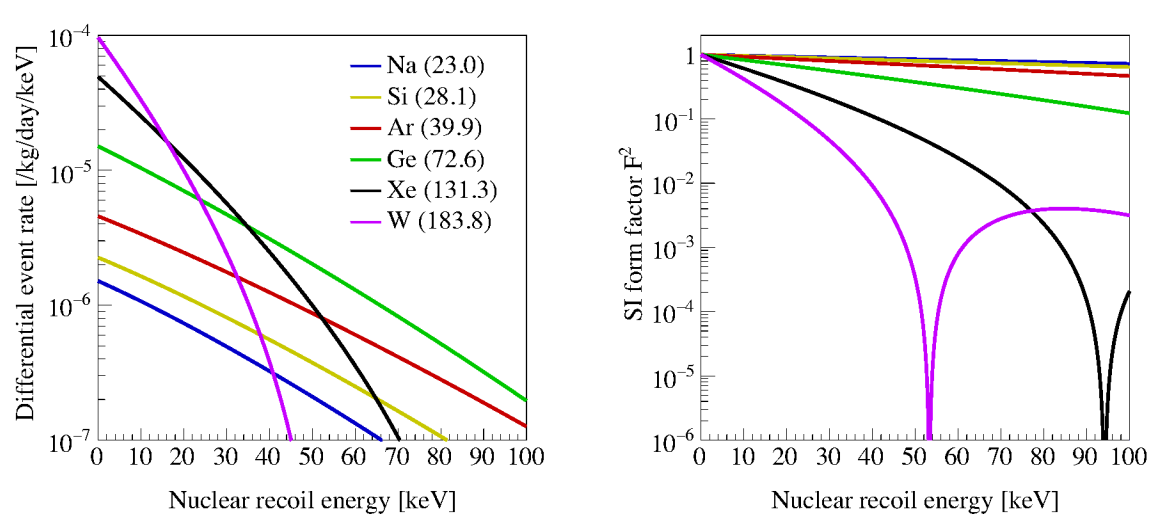
\includegraphics[width=\textwidth]{Figures/LZ/SI_recoil_rate_and_spectra.png}
    \caption{\textbf{Left:} SI nuclear recoil rate for a selection of target elements for a WIMP mass of 100 GeV/c$^2$ and WIMP-nucleon corss section of $\sigma_N=$1 zb and the recommended parameters for the SHM. The averaged atomic mass of each target from natural abundance is in the brackets.
    \textbf{Right:} The Helm form factors for a selection of target nuclei. The key is the same in both plots.
    Both plots are from \cite{LZ_Ibles_LZStats_Thesis_ref}
    \label{fig:si_recoil_and_form_factor}.
           }
\end{figure}
 
\subsection{Form Factors}
\label{sec:form_factors}
\par
One feature which hasn't been mentioned in detail yet is the form factor, $F(q)$.
The form factor contains the physics of the nucleus and is the Fourier transform of the density distribution within.
For SI interactions, this is taken to be the Helm form factor where the nucleus is represented as a solid sphere of radius $r_n$, with a smooth density of nucleons described by a Gaussian of thickness $s$ \cite{helm_form_factor_ref}:
\begin{equation}
    F^2(q) = \bigg( \frac{3j_i(qr_n)}{qr_n} \bigg)^2 e^{-q^2 s^2}
\end{equation}
where $j_i$ is the Bessel function.
\par
%As $r_n \backsim A^{1/3}$ fm, we can see that the WIMP cannot resolve the nucleus as a point-like object.
In the right plot of \autoref{fig:si_recoil_and_form_factor}, the Helm form factors for a selection of popular targets are shown.

\par
For SD interactions, the coupling is not equal between protons and neutrons and so the choice of which nucleus description to use is fairly important.
Depending on which is used the resultant sensitivity to dark matter can vary by orders of magnitude \cite{wimp_nuclear_model_ref,wimp_sd_form_factor_ref}.


\section{Effective Field Theory} \label{sec:eft_theory}

\par
Given the now decades of searching for SI and SD interactions with no success it is right to ask if the assumptions made there are still best.
There may be other corrections (such as momentum dependence) that are the dominant terms.
It is therefore useful to approach a direct dark matter search in a model independent way - namely via an effective field theory (EFT).
\par
An EFT is allows us to describe an unknown model to an arbitrary accuracy by only described the physics at a given scale \cite{eft_expo_ref}.
We parameterise our model in terms of whatever we like though could be in terms of quantities such as energy, momentum or velocity\footnote{This has rather elegantly been quoted as a way to ``parameterise our ignorance" in \cite{shaunalsum_thesis_ref}}.

\par
In the remainder of this chapter we explore the elastic scattering rates in within this model independent approach.
The broad framework which we will follow is from \cite{Fitzpatrick_2013_ref}.

\subsection{Possible Operators}

\par
We begin our journey by treading the WIMP-nucleon elastic scattering as a four-field interaction comprising of the WIMP field $\chi$, the nucleon field $N$ and the effective operators $\Operator$:
\begin{align}
\begin{split}
    \Lagrangian_{int} &= \chi^{+} \Operator_{\chi} \chi^{-} N^{+} \Operator_{N} N^{-} \\
                      &= \Operator \chi^{+}\chi^{-} N^{+}N^{-}
\end{split}
\label{eq:eft_initial_lagrangian}
\end{align}
Now, we can impose constraints by applying symmetries.
\par
Firstly, any operator must be invariant with respect to constant shift in velocities: Galilean invariant.
This allows gives us four quantities with Galilean invariance: momentum transfer, $\vec{q} = \vec{p}_{\chi 1} - \vec{p}_{\chi 2} = \vec{p}_{N 2} - \vec{p}_{N 1}$, the incident WIMP velocity, $\vec{v}=\vec{v_\chi} - \vec{v}_N$, and the spins of the particles: $\vec{S}_N$ and $\vec{S}_\chi$.

\par
Next we look at energy conservation in the centre of mass frame as it cannot change in the collision.

This allows us to equate the initial energy, $E$:
\begin{align}
    E  = \frac{1}{2}\mu_N v^2
\end{align}
to the final kinetic energy, $E'$:
\begin{align}
\begin{split}
    E' &= \frac{1}{2}\mu_N v'^2 \\
       &= \frac{1}{2}\mu_N (\vec{v} + \frac{\vec{q}}{\mu_N})
\end{split}
\end{align}
where $\mu_N=(m_\chi m_N)/(m_\chi + m_N)$ is the WIMP-nucleon reduced mass.
This leaves us with:
\begin{equation}
    \vec{v}\vec{q} = \frac{q^2}{2\mu_N}
\end{equation}
Finally we want the operators to be real values, corresponding to physical quantities, that is to say, Hermitian.
Neither $\vec{q}$ nor $\vec{v}$ are Hermitian, but can be made so by:
\begin{equation}
\begin{split}
    &\vec{q} \rightarrow i\vec{q} \\
    &\vec{v} \rightarrow \vec{v}^{\bot} = \vec{v} + \frac{\vec{q}}{\mu_N}
\end{split}
\end{equation}
There four quantities make up the complete set of parameters which we need to describe our interaction.
We can then take all of the combinations of these variables to leave us with 15 operators:
\begin{equation}
\begin{array}{lcl}
\Operator_{1}=1_{\chi}1_N, \quad \Operator_{2}=\left(v^{\perp}\right)^{2}, \quad \Operator_{3}=i \vec{S}_{N} \cdot\left(\frac{\vec{q}}{m_N} \times \vec{v}^{\perp}\right) \\ 
\Operator_{4}=\vec{S}_{\chi} \cdot \vec{S}_{N}, \quad \Operator_{5}=i \vec{S}_{\chi} \cdot(\frac{\vec{q}}{m_N} \times \vec{v}^{\perp}) \\ 
\Operator_{6}=\left(\vec{S}_{\chi} \cdot \frac{\vec{q}}{m_N}\right)\left(\vec{S}_{N} \cdot \frac{\vec{q}}{m_N}\right) \\
\Operator_{7}=\vec{S}_{N} \cdot \vec{v}^{\perp}, \quad \Operator_{8}=\vec{S}_{\chi} \cdot \vec{v}^{\perp} \\
\Operator_{9}=i \vec{S}_{\chi} \cdot\left(\vec{S}_{N} \times \frac{\vec{q}}{m_N}\right), \quad \Operator_{10}=i \vec{S}_{N} \cdot \frac{\vec{q}}{m_N} \\ 
\Operator_{11}=i \vec{S}_{\chi} \cdot \frac{\vec{q}}{m_N}, \quad \Operator_{12} =\vec{S}_{\chi} \cdot\left(\vec{S}_{N} \times \vec{v}^{\perp}\right) \\
\Operator_{13} =i\left(\vec{S}_{\chi} \cdot \vec{v}^{\perp}\right)\left(\vec{S}_{N} \cdot \frac{\vec{q}}{m_N}\right) \\ 
\Operator_{14} =i\left(\vec{S}_{\chi} \cdot \frac{\vec{q}}{m_N}\right)\left(\vec{S}_{N} \cdot \vec{v}^{\perp}\right) \\ 
\Operator_{15} =-\left(\vec{S}_{\chi} \cdot \frac{\vec{q}}{m_N}\right)\left(\left(\vec{S}_{N} \times \vec{v}^{\perp}\right) \cdot \frac{\vec{q}}{m_N}\right)
\end{array}
\label{eq:EFT_Operators}
\end{equation}
$\Operator_{1}$-$\Operator_{11}$ can be attributed to the exchange of spin-0 or spin-1 mediators, where as $\Operator_{12}$-$\Operator_{15}$ do not.
Some literature also include $\Operator_{16}=-((\vec{S}_\chi \times \vec{v}^{\bot}) \cdot \vec{q})(\vec{S}_N) \cdot \vec{q})$, though as it is just a linear combination of $\Operator_{12}$ and $\Operator_{15}$ it does not need to be included for the most general description.
Typically $\Operator_{2}$ is disregarded due to the $v^{2}$ dependence and so does not appear in non-relativistic models and has such will be dropped here as well.

\par
Before we continue it is important to note that the couplings to the nucleon components are not necessarily the same as each.
This means that each operator, $\Operator$, really represents 2 operators: $\{proton,neutron\}$ or with isospin dependency $\{isoscalar,isovector\}$.
Protons and neutrons are fairly self-explanatory.
Isoscalar particles are singlets with a total isospin of 0 where as isovector particles are triplet states with a total isospin of 1.
Historically there has been limited consistence, with often the same experiment changing between $\{neutron, proton\}$ basis and $\{isoscalar, isovector\}$ basis between data runs.
The choice for some experiments to adopt the $\{neutron, proton\}$ basis has been driven by similarity in reporting results with the standard spin-dependent analysis.
In the last few years however, $\{isoscale, isovector\}$ basis has become more common, with CDMS, XENON100, DEAP-3600 and PandaX-II all reporting results in this basis \cite{cdms_eft_ref,xenon100_eft_ref,deap3600_eft_ref,pandax_2_eft_ref}.
Therefore, in any evaluation a decision needs to be made as to which approach to use.
The translation is fairly trivial with the coupling constants between isoscalar ($c^0$), isovector ($c^1$), proton ($c^p$) and neutron ($c^n$) given by:
\begin{equation}
\begin{split}
    c_i^0 &= \frac{1}{2}(c_i^p + c_i^n)  \\
    c_i^1 &= \frac{1}{2}(c_i^p - c_i^n) 
\end{split}
\label{eq:eft_iso_to_pn}
\end{equation}
In practical terms, this means that out Lagrangian (\autoref{eq:eft_initial_lagrangian}) requires a slight alteration to:
\begin{equation}
    \mathcal{L}_{int}  = \sum_{\tau = (0,1)} \sum_{i}c^{\tau}_{i} \Operator \chi_1 \chi_2 N_1 N_2
\end{equation}
for $\{isoscalar,isovector\}$ and to:
\begin{equation}
    \mathcal{L}_{int} = \sum_{N = (p,n),(\tau)} \sum_{i}c^{(N)}_{i} \Operator \chi_1 \chi_2 N_1 N_2
\end{equation}
for $\{p,n\}$, where $\tau$ refers to the isospin basis.
A priori we know nothing about the strength of these coefficients, and so we cannot say that we know one operator is more significant than another operator.

\par
Although we have constrained ourselves to elastic scatter, this theory can be trivially extended to the inelastic case by $\vec{v}^{\perp} \rightarrow \vec{v}^{\perp} + \frac{\delta_m}{|\vec{q}|^2}\vec{q}$ \cite{inelastics_eft_ref}.

\subsection{To the Nucleus}
\par
Now in order to relate the theory outlined above to what is observable experimentally we must consider that a dark matter particle interact with nucleons that are bound in nuclei rather than free nucleons.
As such, each $\Operator$ needs to be evaluated inside of the target nucleus, and so inserted between nuclear states.
In order to assist in this, we first decompose $\vec{v}$ of each nucleon into the velocity with respect to the centre of mass $\vec{v}_{N}$ and the nucleus centre of mass velocity $\vec{v}_{A}$.
This can also be done for the transverse velocity $\vec{v}^{\perp}$ where $\vec{v}^{\perp}_{A}=\vec{v}_A + \vec{q}/2\mu_{A}$ and $\vec{v}^{\perp}_{N}=-1/2(\vec{v}_{N} + \vec{v}^{'}_{N})$.

\par
Putting this decomposition together we can define our interaction Lagrangian as a linear combination of these operators in the centre of mass frame of the nucleus:
\begin{equation}
\begin{split}
    \mathcal{L}_{int}\quad  & =\quad c_1 \\
             & +\quad ic_3 \vec{S}_{N} \cdot ( \vec{q} \times \vec{v}^{\perp}_{A} ) + ic_3 \vec{S}_{N}
             \cdot( \vec{q} \times \vec{v}^{\perp}_{N} ) \\
             & +\quad c_4 \vec{S}_{\chi} \cdot \vec{S}_{N} \\
             & +\quad ic_5 \vec{S}_{\chi} \cdot(\vec{q} \times \vec{v}^{\perp}_{A}) + ic_5 \vec{S}_{\chi} \cdot ( \vec{q} \times \vec{v}^{\perp}_{N} ) \\
             & +\quad c_6 ( \vec{S}_{\chi} \cdot \vec{q} ) (\vec{S}_{N} \cdot \vec{q} ) \\
             & +\quad c_7 \vec{S}_{N} \cdot \vec{v}^{\perp}_{A} + c_7 \vec{S}_{N} \cdot \vec{v}^{\perp}_{N} \\
             & +\quad c_8 \vec{S}_{\chi} \cdot \vec{v}^{\perp}_{A} + c_8 \vec{S}_{\chi} \cdot \vec{v}^{\perp}_{N} \\
             & +\quad ic_9 \vec{S}_{\chi} \cdot ( \vec{S}_{N} \times \vec{q} ) \\
             & +\quad ic_{10} \vec{S}_{N} \cdot \vec{q} \\
             & +\quad ic_{11} \vec{S}_{\chi} \cdot \vec{q} \\
             & +\quad c_{12} \vec{S}_{\chi} \cdot ( \vec{S}_{N} \times \vec{v}^{\perp}_{A} ) + c_{12} \vec{S}_{\chi} \cdot ( \vec{S}_{N} \times \vec{v}^{\perp}_{N} ) \\
             & +\quad ic_{13} ( \vec{S}_{\chi} \cdot \vec{v}^{\perp}_{A} ) ( \vec{S}_{N} \cdot \vec{q} ) + ic_{13} ( \vec{S}_{\chi} \cdot \vec{v}^{\perp}_{N} ) ( \vec{S}_{N} \cdot \vec{q} ) \\
             & +\quad ic_{14} ( \vec{S}_{\chi} \cdot \vec{q} ) ( \vec{S}_{N} \cdot \vec{v}^{\perp}_{A} ) + ic_{14} ( \vec{S}_{\chi} \cdot \vec{q} ) ( \vec{S}_{N} \cdot \vec{v}^{\perp}_{N} ) \\
             & -\quad c_{15}(\vec{S}_{\chi} \cdot \vec{q}) ( ( \vec{S}_{N} \times \vec{v}^{\perp}_{A} ) \cdot \vec{q} ) - c_{15} ( \vec{S}_{\chi} \cdot \vec{q} ) ( ( \vec{S}_{N} \times \vec{v}^{\perp}_{N} ) \cdot \vec{q} )
\end{split}
\label{eq:eft_operator_lagrangian_com}
\end{equation}
The equation above has been written such that it is only in terms of the degrees of freedom available to the nucleus ($\vec{S}_{N},\vec{v}^{\perp}_{N}$).
This shows us that there are just three scalar quantities: 
\begin{equation}
    1, \vec{v}^{\perp}_{N} \cdot \vec{v}^{\perp}_{N}, \text{and} \vec{S}_{N} \cdot \vec{v}^{\perp}_{N}
\end{equation}
and three nucleus dependent currents:
\begin{equation}
    \vec{S}_{N}, \vec{v}^{\perp}_{N}, \text{and} \vec{S}_{N} \times \vec{v}^{\perp}_{N}
\end{equation}
that can can be created.
As before we will disregard $\vec{v}^{\perp}_{N} \cdot \vec{v}^{\perp}_{N}$ as it does not appear in the lowest order, leaving us with five unique nuclear charges and currents that can couple to our dark matter.

\par
We can rearrange our Lagrangian (\autoref{eq:eft_operator_lagrangian_com}) to be linear combinations of these:
\begin{equation}
\begin{split}
    \mathcal{L}_{int}\quad  & =\quad \Bigl\{ c_1 + ic_{5}\vec{S}_{\chi} \cdot (\vec{q} \times \vec{v}^{\perp}_{A}) + c_8 (\vec{S}_{\chi} \cdot \vec{v}^{\perp}_{A}) + ic_{11} (\vec{S}_{\chi} \cdot \vec{q} ) \Bigl\} \\
                            & +\quad \Bigl\{ c_7 + ic_{14}(\vec{S}_{\chi} \cdot \vec{q}) \Bigl\} \cdot [\vec{S}_{N} \cdot \vec{v}^{\perp}_{N}] \\
                            & +\quad \Bigl\{ ic_3 (\vec{q} \times \vec{v}^{\perp}_{A}) + c_4\vec{S}_{\chi} + c_6 (\vec{S}_{\chi} \cdot \vec{q} ) \vec{q} + c_7 \vec{v}^{\perp}_{A} + ic_9 ( \vec{q} \times \vec{S}_{\chi} ) + ic_{10} \vec{q} \\
                            & \qquad+ c_{12} (\vec{v}^{\perp}_{A} \times \vec{S}_{\chi}) + ic_{13} (\vec{v}^{\perp}_{A} \cdot \vec{S}_{\chi}) \vec{q} + ic_{14}(\vec{q} \cdot \vec{S}_{\chi})\vec{v}^{\perp}_{A} - c_{15}(\vec{S}_{\chi} \cdot \vec{q}) \vec{q} \Bigl\} \cdot [\vec{S}_{N}] \\
                            & +\quad \Bigl\{ ic_5 (\vec{S}_{\chi} \times \vec{q}) + c_8 \vec{S}_{\chi} \Bigl\} \cdot [\vec{v}^{\perp}_{N}] \\
                            & +\quad \Bigl\{ ic_3 \vec{q} + c_{12} \vec{S}_{\chi} - ic_{13} (\vec{q} \times \vec{S}_{\chi}) - c_{15} (\vec{q} \cdot \vec{S}_{\chi}) \vec{q} \Bigl\} \cdot [\vec{S}_{N} \times \vec{v}^{\perp}_{N}] 
\end{split}
\label{eq:eft_operator_lagrangian_charges_and_currents}
\end{equation}
In \autoref{eq:eft_operator_lagrangian_charges_and_currents} each term inside the curly brackets which can be explicitly names:
\begin{equation}
\begin{split}
    l_0  & = c_1 - ic_5 \vec{v}^{\perp}_{A} \cdot(\vec{q} \times \vec{S}_\chi) + c_8 \vec{S}_\chi \cdot \vec{v}^{\perp}_{A} + ic_{11} \vec{S}_\chi \cdot \vec{q} \\
    l^A_0 &= c_7 + ic_{14} (\vec{S}_\chi \cdot \vec{q}) \\
    \vec{l}_5 &= \frac{1}{2} \big[ ic_3 (\vec{q} \times \vec{v}^{\perp}_{A}) + c_4 \vec{S}_\chi + c_6 (\vec{S}_\chi \cdot \vec{q}) \vec{q} + c_7 \vec{v}^{\perp}_{A} + ic_9 (\vec{q} \times \vec{S}_\chi) + ic_{10} \vec{q} \\
    &\qquad+ c_12 (\vec{v}^{\perp}_{A} \times \vec{S}_\chi) + ic_{13} (\vec{v}^{\perp}_{A} \cdot \vec{S}_\chi) \vec{q} + ic_{14}(\vec{q} \cdot \vec{S}_\chi)\vec{v}^{\perp}_{A} - c_{15} (\vec{S}_\chi \cdot \vec{q} ) \vec{q} \bigg] \\
    \vec{l}_M &= ic_5 (\vec{S}_\chi \times \vec{q}) - c_8 \vec{S}_\chi \\
    \vec{l}_E &= -\frac{1}{2} \bigg[ c_3 + ic_{12} \vec{S}_\chi - c_{13} (\vec{q} \times \vec{S}_\chi) - ic_{15} (\vec{q} \cdot \vec{S}_{\chi}) \vec{q} \bigg] \vec{q}
\end{split}
\label{eq:eft_operator_lagrangian_charges_and_currents}
\end{equation}
This allows the Lagrangian to be written as:
\begin{equation}
    \mathcal{L} = l_01 + l_0^A[-2\vec{v}^{\perp}_N \cdot \vec{S}_N] + \vec{l}_{5} \cdot [2\vec{S}_N] + \vec{l}_{M} \cdot [-\vec{v}^{\perp}_N] + \vec{l}_{E} \cdot [2i\vec{v}^{\perp}_N \times \vec{S}_{N} ]
\end{equation}
We still have only defined a WIMP-nucleon interaction, and so we need to go further to obtain a WIMP-nucleus interaction: which is just the sum of the contributions from each nucleon:
\begin{equation}
    \mathcal{L}^{\text{Nucleus}}_{\text{int}} = \sum_{i}^{A} \mathcal{L}^{N_i}_{\text{int}}
\end{equation}
In order to simplify the scattering amplitude evaluation, and to maintain consistency with literature \cite{Fitzpatrick_2013_ref}, we will apply a set of transformations to go from momentum space to coordinate space:
\begin{equation}
    \begin{split}
        -\vec{v}^{\perp}_{N_i} &= \frac{\vec{p}_{N_i} + \vec{p}^{'}_{N_i}}{2m_N} \rightarrow \frac{1}{2m_N}i \Bigg( \vec{\nabla}\delta(\vec{r - \vec{r}_i}) - \delta(\vec{r} - \vec{r}_i) \vec{\nabla} \Bigg) \\
        \vec{S}_{N_i} &= \vec{\sigma}(i) \\
        1 &\rightarrow \delta(\vec{r} - \vec{r}_i)
    \end{split}
\end{equation}
where $\vec{r}_i$ is the position of the $i^{th}$ nucleon with respect to the centre of mass of the nuclei, $\vec{r}$ is the position of the dark matter particle with respect to the centre of mass of the nuclei and $\vec{\sigma}(i)$ is the spin operator in terms of the Pauli spin matrices.
$\vec{p}_{N_i}$ and $\vec{p}^{'}_{N_i}$ are the initial and final momenta of the $i^{th}$ nucleon.
By including a plane wave of the form $e^{-i \vec{q}\cdot \vec{r}}$ to each term we are able to consider a nucleon at every location.
This leaves us with a Hamiltonian density for the WIMP-nucleus interaction of:
\begin{equation}
\begin{split}
    \mathcal{H}(\vec{r})\quad  & =\quad \sum^{A}_{i=1} l_{0}(i) \delta(\vec{r} - \vec{r}_i) e^{-i\vec{q}\cdot \vec{r}} \\
                               & +\quad  \sum^{A}_{i=1} l^A_0 (i) \frac{i}{2m_N} \Bigg[ \vec{\nabla} \cdot \vec{\sigma}(i) \delta(\vec{r} - \vec{r}_i) e^{-i\vec{q}\cdot \vec{r}} - e^{-i\vec{q}\cdot \vec{r}} \delta(\vec{r} - \vec{r}_i) \vec{\sigma}(i) \cdot \vec{\nabla} \Bigg] \\
                               & +\quad  \sum^{S}_{i=1} \vec{l}_5 (i) \cdot \vec{\sigma}(i)\delta(\vec{r} - \vec{r}_i)e^{-i\vec{q}\cdot \vec{r}} \\
                               & +\quad  \sum^{A}_{i=1} \vec{l}_M (i) \cdot \frac{i}{2m_N} \Bigg[ \vec{\nabla} \delta(\vec{r} - \vec{r}_i)e^{-i\vec{q}\cdot \vec{r}} - e^{-i\vec{q}\cdot \vec{r}}\delta(\vec{r} - \vec{r}_i)\vec{\nabla} \Bigg] \\
                               & +\quad \sum^{A}_{i=1} \vec{l}_E (i) \cdot \frac{1}{2m_N} \Bigg[ \vec{\nabla} \times \vec{\sigma}(i)\delta(\vec{r} - \vec{r}_i)e^{-i\vec{q}\cdot \vec{r}} + e^{-i\vec{q}\cdot \vec{r}}\delta(\vec{r} - \vec{r}_i) \vec{\sigma}(i) \times \vec{\nabla} \Bigg]
\end{split}
\label{eq:eft_hamiltonian_density}
\end{equation}

\par
We can then integrate over the nucleon positions to get the Hamiltonian, H.
This as it turns out is the easiest step it just contracting the delta functions and replacing $e^{-i\vec{q}\cdot \vec{r}}$ with $e^{-i\vec{q}\cdot \vec{r}_i}$.
Which leaves us with:
\begin{equation}
\begin{split}
    H\quad & =\quad \sum^{A}_{i=1} l_{0}(i) e^{-i\vec{q}\cdot \vec{r}_i} \\
           & +\quad \sum^{A}_{i=1} l^A_0 (i) \frac{i}{2m_N} \Bigg[ \vec{\nabla} \cdot \vec{\sigma}(i) e^{-i\vec{q}\cdot \vec{r}_i} - e^{-i\vec{q}\cdot \vec{r}_i} \vec{\sigma}(i) \cdot \vec{\nabla} \Bigg] \\
           & +\quad \sum^{S}_{i=1} \vec{l}_5 (i) \cdot \vec{\sigma}(i) e^{-i\vec{q}\cdot \vec{r}_i} \\
           & +\quad \sum^{A}_{i=1} \vec{l}_M (i) \cdot \frac{i}{2m_N} \Bigg[ \vec{\nabla} e^{-i\vec{q}\cdot \vec{r}_i} - e^{-i\vec{q}\cdot \vec{r}_i}\vec{\nabla} \Bigg] \\
           & +\quad \sum^{A}_{i=1} \vec{l}_E (i) \cdot \frac{1}{2m_N} \Bigg[ \vec{\nabla} \times \vec{\sigma}(i)e^{-i\vec{q}\cdot \vec{r}_i} + e^{-i\vec{q}\cdot \vec{r}_i} \vec{\sigma}(i) \times \vec{\nabla} \Bigg]
\end{split}
\label{eq:eft_hamiltonian}
\end{equation}
We are then able to calculate the scattering amplitude for the interaction in the same way as before for the SI case, by averaging over the initial spins and summing over the final spins:
\begin{equation}
    | \mathcal{M} |^2  = |\langle j_\chi,M_\chi;j_N M_N | H | j_\chi,M_\chi;j_N M_N \rangle |^2
\end{equation}
Before we show the explicit result of this, we should first look back towards our Hamiltonian.
It is simply comprised of a number of terms, each of which contain the couple constant for a single EFT operator.
We are able to express our scattering matrix element in a similar fashion: as the sum of a number of smaller terms, each of which involving a single operator.
In this case, we can write it as:
\begin{equation}
    \frac{1}{(2j_A + 1)}\frac{1}{(2j_\chi + 1)} \sum_{spins} |\mathcal{M}|^2 \equiv
    \frac{m_A^2}{m_N^2} \sum_{i,j=1}^{15} \sum_{a,b=0,1} c_i^{a}c_{j}^{b} F_{ij}^{a,b} (v^2,q^2)
    \label{eq:eft_scattering_amplitude_in_terms_of_operator_form_factors}
\end{equation}
In \autoref{eq:eft_scattering_amplitude_in_terms_of_operator_form_factors} we have introduced $F_{ij}^{a,b}(v^2,q^2)$, which is the unique form factor associated to each nucleus and combination of WIMP-nucleon operators.
\par
The actual evaluation of these nuclear form factors are not particularly straight forward, and with uncertainties on which nuclear model is the most accurate still debated, can have a non-negligible impact on any dark matter sensitivity.
The approach adopted in \cite{Fitzpatrick_2013_ref} is to perform a multipole decomposition where the following identities are used:
\begin{equation}
\begin{split}
e^{i \vec{q} \cdot \vec{r}_i}\;&=\;\sum_{J=0}^{\infty} \sqrt{4 \pi} \sqrt{2 J+1} i^J j_J\left(q r_i\right) Y_{J 0}\left(\Omega_{r_i}\right) \\
\hat{e}_\lambda e^{i \vec{q} \cdot \vec{r}_i} \; &= \; 
\begin{dcases}
\sum_{J=0}^{\infty} \sqrt{4 \pi} \sqrt{2 J+1} i^{J-1} \frac{\vec{\nabla}_i}{q} j_J\left(q r_i\right) Y_{J 0}\left(\Omega_{r_i}\right) & \lambda=0 \\
\sum_{J \geq 1}^{\infty} \sqrt{2 \pi} \sqrt{2 J+1} i^{J-2}\left[\lambda j_J\left(q r_i\right) \vec{Y}_{J J 1}^\lambda\left(\Omega_{r_i}\right)+\frac{\vec{\nabla}_i}{q} \times j_J\left(q r_i\right) \vec{Y}_{J J 1}^\lambda\left(\Omega_{r_i}\right)\right] & \lambda=\pm 1
\end{dcases}
\end{split}
\label{eq:eft_multipole_expansion}
\end{equation}
In the above equation, $j_J$ is a spherical Bessel function, $Y_{LM}$ is a spherical harmonic function, and $\vec{Y}^{\lambda}_{LM}$ is a vector spherical harmonic.
$\Omega$ is the direction of the vector $\vec{r}_i$.
The reason for this multipole expansion approach is that it allows for exploitation of the assumption of CP and parity symmetry in the nuclear ground state.
Not only do most multipoles vanish under this assumption, but the majority of off-diagonal terms disappear as well.
During this expansion the intermittent expressions are not friendly and as such are not included here, but if the reader is curious they are directed to Appendix A.1 of \cite{Fitzpatrick_2013_ref}, though it is also recommended that both \cite{weak_multipole_expansion_ref} and \cite{semileptonic_multipole_expansion_ref} be read for an improved understanding of the calculation.
\par
We can now arrive at the dark matter scattering amplitude:
\begin{equation}
\begin{split}
    | \mathcal{M} |^2  &= |\langle j_\chi,M_\chi;j_N M_N | H | j_\chi,M_\chi;j_N M_N \rangle |^2 \\
    &= 4 \pi \sum_{i=1}^{A} \left[ \sum_{J=1,3,...}^{\infty} | \langle J_i||\vec{l}_5 \cdot \hat{q} \Sigma_{J}^{''}(q) || J_i \rangle |^2 \right. \\
    &\quad+ \sum_{J=0,2,...}^{\infty} \Bigl\{ | \langle J_i||l_0 M_J (q) || J_i \rangle |^2 + | \langle J_i||\vec{l}_E \cdot \hat{q} \frac{q}{m_N} \Phi^{''}_{J} (q) || J_i \rangle |^2 \\
    &\qquad\qquad\qquad+ 2\text{Re} \Bigl[ \langle J_i || \vec{l}_E \cdot \hat{q} \frac{q}{m_N} \Phi^{''}_{J}(q) || J_i\rangle \langle J_i||l_0 M_{J}(q)||J_i\rangle^*\Bigl] \Bigl\} \\
    &\quad+ \frac{q^2}{2m^2_N} \sum_{J=2,4,...}^{\infty} \Bigl( \langle J_i || \vec{l}_E \tilde{\Phi}_{J}(q) || J_i \rangle \cdot \langle J_i || \vec{l}_M \Delta_{J}(q) || J_i \rangle^* - |\langle J_i || \vec{l}_m \cdot \hat{q}\Delta_{J}(q) ||J_i \rangle |^2 \Bigl) \\
    &\quad+ \sum_{J=1,3,...}^{\infty} \Bigl\{ \frac{q^2}{2m^2_N} \Bigl( \langle J_i || \vec{l}_M \Delta_{J}(q) || J_i \rangle \cdot \langle J_i || \vec{l}_5 \cdot \hat{q}\Delta_{J}(q) || J_i \rangle |^2 \Bigl) \\
    &\qquad\qquad\qquad+ \frac{1}{2} \Bigl( \langle J_i|| \vec{l}_5 \Sigma^{'}_{J}(q) || J_i \rangle \cdot \langle J_i||\vec{l}_5 \Sigma^{'}_{J}(q) || J_i \rangle^2 - |\langle J_i||\vec{l}_5 \cdot \hat{q} \Sigma^{'}_{J} || J_i \rangle |^2 \Bigl) \\
    &\qquad\qquad\qquad+ 2\text{Re} \Bigl[ i\hat{q} \cdot \langle J_i || \vec{l}_M \frac{q}{m_N} \Delta_{J}(q) || J_i \rangle  \times \langle J_i||\vec{l}_{5} \Sigma^{'}_{J}(q) || J_i \rangle^* \Bigl] \Bigl\} \Biggr] 
\end{split}
\label{eq:eft_scattering_amplitude}
\end{equation}
In \autoref{eq:eft_scattering_amplitude} we have introduced six nuclear responses, $M,\Sigma^{'},\Sigma^{''},\nabla,\tilde{\Phi}^{'},\Phi^{''}$. 
Each of which can be written in terms of spherical harmonics previously defined:
\begin{equation}
\begin{split}
    M_{JM}(qr) &\equiv j_J(qr)Y_J M(\Omega_r) \\
    \vec{M}^{M}_{JL} &\equiv j_L (qr) \vec{Y}_{JLM}
\end{split}    
\end{equation}
This allows us to write these nuclear responses as:
\begin{equation}
\begin{split}
    \Delta_{JM}(q\vec{r})\quad &\equiv\quad \vec{M}_{JJ}^{M}(q\vec{r}) \cdot \frac{1}{q}\vec{\nabla} \\
    \Sigma^{'}_{JM}(q\vec{r})\quad &\equiv\quad -i \bigg\{ \frac{1}{q} \vec{\nabla} \times \vec{M}^{M}_{JJ}(q\vec{r}) \bigg\} \cdot \vec{\sigma} \\
    & =\quad (J(J + 1))^{-1}\bigg\{-\sqrt{J}\vec{M}^{M}_{JJ+1}(q\vec{r}) + \sqrt{J+1} \vec{M}^{M}_{JJ-1}(q\vec{r}) \bigg\} \cdot \vec{\sigma} \\
    \Sigma^{''}_{JM}(q\vec{r})\quad &\equiv\quad \bigg\{\frac{1}{q}\vec{\nabla}\vec{M}^{M}_{JJ}(q\vec{r}) \bigg\} \cdot \vec{\sigma} \\
    & =\quad (J(J + 1))^{-1} \bigg\{-\sqrt{J+1}\vec{M}^{M}_{JJ+1}(q\vec{r}) + \sqrt{J}\vec{M}^{M}_{JJ-1}(q\vec{r}) \bigg\} \cdot \vec{\sigma} \\
    \tilde{\Phi}^{'}_{JM}(q\vec{r})\quad &\equiv\quad \bigg( \frac{1}{q}\vec{\nabla} \times \vec{M}^{M}_{JJ}(q\vec{r}) \bigg) \cdot \bigg( \vec{\sigma} \times \frac{1}{q} \vec{\nabla} \bigg) + \frac{1}{2}\vec{M}^{M}_{JJ}(q\vec{r}) \cdot \vec{\sigma} \\
    \Phi^{''}_{JM}(q\vec{r})\quad &\equiv\quad i \bigg( \frac{1}{q}\vec{\nabla}\vec{M}^{M}_{JJ}(q\vec{r}) \bigg) \cdot \bigg( \vec{\sigma} \times \frac{1}{q}\vec{\nabla} \bigg)
\end{split}
\label{eq:eft_nuclear_response_operators}
\end{equation}
Each of these nuclear response operators are directly from electroweak physics - or with simple modifications for which the reader is directed to \cite{Fitzpatrick_2013_ref}.
\par
The form factors we saw in \autoref{eft_scattering_amplitude_in_terms_of_operator_form_factors} can be constructed as a linear combination of nuclear form factors that are associated with these nuclear responses:
\begin{equation}
    F^{a,b}_{ij} = \sum_{k=M,\Sigma^{''},\Sigma^{'},\Delta, \Phi^{''},\tilde{\Phi}^{'}} a_{ijk}(j_\chi,v^2,q^2) F_{k}^{(a,b)}
    \label{eq:eft_form_factor_relation_to_nuclear_form_factors}
\end{equation}
All parameters which depend on our dark matter, included mass, spin and relative velocity, are all contained within the coefficients $a_{ijk}$.
This leaves the nuclear form factors as dependent exclusively on the target nucleus.
Each nuclear form factor is defined as:
\begin{equation}
    F^{a,b}_X(q^2) \equiv \frac{4 \pi}{2j + 1} \sum^{2j+1}_{J=1} \langle j || X^{a}_{j} || j \rangle \langle j || X^{b}_{j} || \rangle 
\end{equation}
assuming that there is no interference or, if there is interference between responses:
\begin{equation}
    F^{a,b}_{X,Y}(q^2) \equiv \frac{4 \pi}{2j + 1} \sum^{2j+1}_{J=1} \langle j || X^{a}_{j} || j \rangle \langle j || Y^{b}_{j} || \rangle 
\end{equation}
which is allowed between $M$ and $\Phi^{''}$ and between $\Sigma^{'}$ and $\Sigma^{''}$.

\par
For calculated form factors the reader is directed towards \cite{Fitzpatrick_2013_ref, dmformfactor_ref, nicolelarsen_thesis_ref}.
However, most of these only show the \{$n,p$\} result, so below is provided the conversion to those needed for \{$isoscalar,isovector$\}:
\begin{align}
    \begin{split}
        F_{i,j}^{00}    &= \frac{1}{4} \left( F_{i,j}^{(n,n)} + F_{i,j}^{(p,p)} + F_{i,j}^{(p,n)} + F_{i,j}^{n,p} \right) \\
        F_{i,j}^{01}    &= \frac{1}{4} \left( -F_{i,j}^{(n,n)} + F_{i,j}^{(p,p)} - F_{i,j}^{(p,n)} + F_{i,j}^{n,p} \right) \\
        F_{i,j}^{10}    &= \frac{1}{4} \left( -F_{i,j}^{(n,n)} + F_{i,j}^{(p,p)} + F_{i,j}^{(p,n)} - F_{i,j}^{n,p} \right) \\
        F_{i,j}^{11}    &= \frac{1}{4} \left( F_{i,j}^{(n,n)} + F_{i,j}^{(p,p)} - F_{i,j}^{(p,n)} - F_{i,j}^{n,p} \right)
    \end{split}
\end{align}

\subsection{Scattering Rate}
\par
Now that we have all of the tools needed to calculate the scattering amplitude for any interaction in our theory we can relate this to a scattering rate.
Fortunately for us this is the simplest step so far, and one which we've already done for the SI interaction:
\begin{equation}
    \frac{dR}{dE_R} = N_T \frac{\rho_{\chi}}{32 \pi m_\chi^3 m_A} \int_{v>v_{min}} \frac{1}{v}f(\vec{v}) | \mathcal{M} |^2 d^3 v 
    \label{eq:eft_differential_cross_section}
\end{equation}
In this equation, the spin contributions of the initial states are averaged and the final states are summed.
It should be noted that in \autoref{eq:eft_differential_cross_section} a factor $1/(4m_\chi m_A)^2$ has been introduced.
This is to follow the conversion set out in \cite{dmformfactor_ref}, where this factor is included to account for the normalisation required to match the relativistic WIMP-nucleon interaction operators to the non-relativistic terms.

Combining \autoref{eq:eft_scattering_amplitude_in_terms_of_operator_form_factors} with \autoref{eq:eft_differential_cross_section} give us our final differential rate:

\begin{equation}
    \frac{dR}{dE_R} = N_T \frac{\rho_{\chi} m_A}{32 \pi m_\chi^3 m_N^2} \int_{v>v_{min}} \frac{f(\vec{v})}{v} \sum_{i,j=1}^{15} \sum_{a,b=0,1} c_i^a c_j^b \sum_{k=M,\Sigma^{''},\Sigma^{'},\Delta, \Phi^{''},\tilde{\Phi}^{'}} a_{i,j,k}F_{k}^{(a,b)} d^3 v
    \label{eq:final_eft_differential_cross_section}
\end{equation}

\subsection{EFT Searches}
\par
Due to the complexity of evaluating the nuclear form factors and the uncertainties in the parameters, direct dark matter searches have generally focused on setting limits on the individual operator coupling constants.
This is performed by simply evaluating the scattering amplitude assuming a single operator.
Prior to the work presenting in \autoref{chap:eft_work}, the current best limits come from XXX, which was a study performed in the \{$neutron,proton$\} basis.

\par
It is interesting to note however that a recent publication by Panda-X extended this to a generalised spin analysis, using linear combinations of the operators.
Most notably:
\begin{equation}
\begin{split}
    \text{WIMP Magnetic Moment, nucleon vector current} & -\frac{q^2}{2m_\chi m_M}\Operator_1 + \frac{2m_N}{m_M}\Operator_5 - \frac{2m_N}{m_M}(\frac{q^2}{m_N^2}\Operator_4 - \Operator_6) \\
    \text{WIMP electric dipole moment, nucleon vector current} & \frac{2m_N}{m_M}\Operator_{11} \\
    \text{WIMP magnetic moment, nucleon magnetic moment} & 4(\frac{q^2}{m_M^2}\Operator_4 - \frac{m_N^2}{m_M^2}\Operator_6)
\end{split}
\end{equation}
The new quantity introduced here, $m_M$, is just the strength of the WIMP and nucleon moments being coupled, and is taken to be $m_M \sim m_N$.

\par
Writing optimistically, we can also excess our differential rate as:
\begin{equation}
    \frac{d\sigma}{dE_R} \approx G_F^2 \sum_{i} R_i (\vec{v}^{\perp 2}, \frac{\vec{q}^2}{m_N^2}) W_i(q^2b^2)
\end{equation}
where $W_i(q^2b^2)$ encompasses the nuclear tensor and $R_i (\vec{v}^{\perp 2}, \frac{\vec{q}^2}{m_N^2})$, is the WIMP tensor, containing all of the dark matter particle physics.
In a direct dark matter experiment, this can be varied to change the nuclear charge, spin, isospin to determine $R_i$.
As there are many different direct dark matter experiment, each with different target nuclei, each with different properties and sensitivities, they combine together to contain the dark matter.
